\icode{N20L-MVV-MU-L3-261111-001}
\nceeID[4]{2020山东}{11}
（多选）
如图所示，质量为\(M\)的物块\(A\)放置在光滑水平桌面上，右侧连接一固定于墙面的水平轻绳，左侧通过一倾斜轻绳跨过光滑定滑轮与一竖直轻弹簧相连。现将质量为\(m\)的钩码\(B\)挂于弹簧下端，当弹簧处于原长时，将\(B\)由静止释放，当\(B\)下降到最低点时(未着地)，\(A\)对水平桌面的压力刚好为零。轻绳不可伸长，弹簧始终在弹性限度内，物块\(A\)始终处于静止状态。以下判断正确的是\paren[]

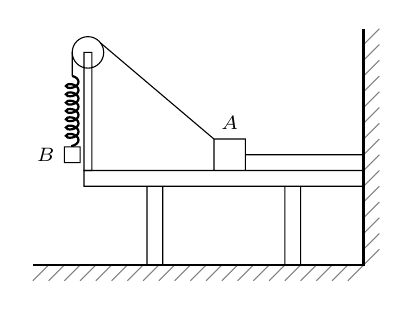
\begin{tikzpicture}[font=\scriptsize]
	\draw (-.05,0) rectangle(.05,1.5) (0,1.5) circle(.2);
	\draw (-.05,0) rectangle(3.5,-.2) (.75,-.2) rectangle(.95,-1.2) (2.5,-.2) rectangle(2.7,-1.2) (1.6,0) rectangle (2,.4) (1.6,.4)--(.16,1.62) (2,.2)--(3.5,.2) (-.2,1.5)--(-.2,1.2) (-.3,.3) rectangle(-.1,.1);
	\draw[thick,decoration={aspect=.6,segment length=3,amplitude=.8mm,coil},decorate] (-.2,1.2)--(-.2,.3);
	\foreach \x in {-.7,-.5,...,3.3}
		\draw[gray] (\x,-1.4)--++(.2,.2);
	\foreach \y in {-1.2,-1,...,1.6}
		\draw[gray] (3.5,\y)--++(.2,.2);
	\draw[thick] (-.7,-1.2)--(3.5,-1.2)--(3.5,1.8);
	\node at(-.3,.2)[left]{\(B\)};
	\node at(1.8,.4)[above]{\(A\)};
\end{tikzpicture}
\begin{choices}
	\item\(M < 2m\)
	\item\(2m < M < 3m\)
	\item 在\(B\)从释放位置运动到最低点的过程中，所受合力对\(B\)先做正功后做负功
	\item 在\(B\)从释放位置运动到速度最大的过程中，\(B\)克服弹簧弹力做的功等于\(B\)机械能的减少量
\end{choices}
\begin{answer}
    AC\qquad 提示：
\end{answer}